\section{Tableau de bord}
\noindent
Le tableau de bord (ou dashboard en anglais) est un outil qui permet à plusieurs collaborateurs de suivre l’avancée d’un projet. Il présente de manière synthétique tous les éléments et indicateurs clés qui permettent à la fois :
\begin{itemize}
	\item D’organiser le jalonnage, lister les tâches et de les assigner aux différentes parties prenantes au projet.
	\item De prendre des décisions et de mettre des correctifs en place quand des alertes sont remontées.
\end{itemize}


\subsection{Les indicateurs de performance}
\noindent
Un indicateur de performance est un mesure ou un ensemble de mesures d'un aspect spécifique et essentiel de la performance globale de l'organisation.
Dans cette section, nous allons présenter les différents indicateurs que nous avons choisis pour le tableau de bord de l'admin. Nous remplissons le tableau ~\ref{tab:kpi} avec:
\begin{itemize}
	\item \large\textbf{Indicateur de performance (KPI):} Le nom de l'indicateur
	\item \large\textbf{Objectif:} l'importance ou la signification de l'indicateur
	\item \large\textbf{Visualisation:} la manière dont l'indicateur sera affiché et le type de graphique approprié pour cet indicateur.
	\item \large\textbf{Spécifications:} Les détails descriptifs concernant chaque KPI.
\end{itemize}

\newpage
\begin{table}[H]
    \centering
    \renewcommand{\arraystretch}{1.5}
    \begin{tabular}{|>{\bfseries}m{4cm}|m{4cm}|m{4cm}|m{4cm}|}
        \hline
        \rowcolor{blue!50}
        \textbf{KPI} & \textbf{Objectif} & \textbf{Visualisation} & \textbf{Spécification} \\
        \hline
        Score de similarité de recherche & Mesurer le score de similarité entre le terme de recherche et les produits & Diagramme à Bandes & Similarité entre le terme de recherche et les produits  \\
        \hline
        Les mots les plus recherché & Mesure les mots les plus recherché dans le site  & Diagramme Circulaire & Nombre de mots (en pourcentage) recherché par rapport au total des recherches \\
        \hline
    \end{tabular}
    \caption{Tableau des KPIs}
    \label{tab:kpi}
\end{table}

\section{Réalisation}
\noindent
Dans cette section nous présentons le tableau de bord pour notre administrateur développé durant le Sprint 3, ainsi que l'interface de modification des paramétres de recherche des produits, et bien sûr l'interface d'authentification. \\
\newpage
\noindent
La figure ~\ref{fig:admindashboard} visualise les KPIs mentionné précédemment dans le tableau ~\ref{tab:kpi}

\begin{figure}[H]
    \centering
    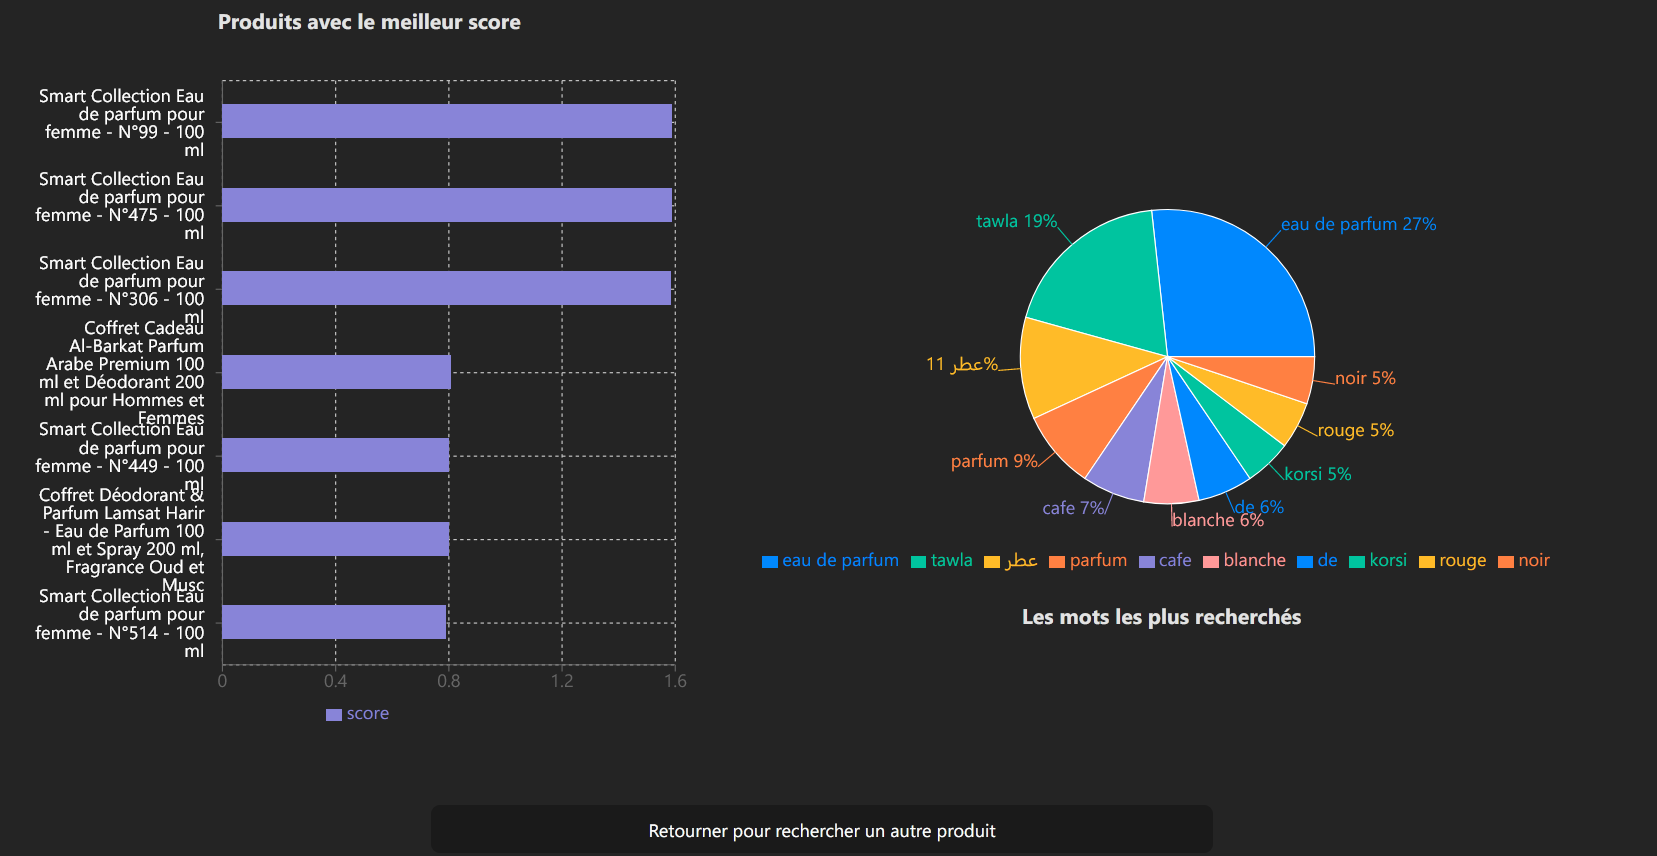
\includegraphics[width=1\textwidth]{logos/dashboard.png}
    \caption{Interface de Tableau de bord de l'administrateur}
    \label{fig:admindashboard}
\end{figure}

\newpage
\noindent
La figure ~\ref{fig:knnsearchform} illustre le formulaire de modification de paramétres de recherche pour l'administrateur.

\begin{figure}[H]
    \centering
    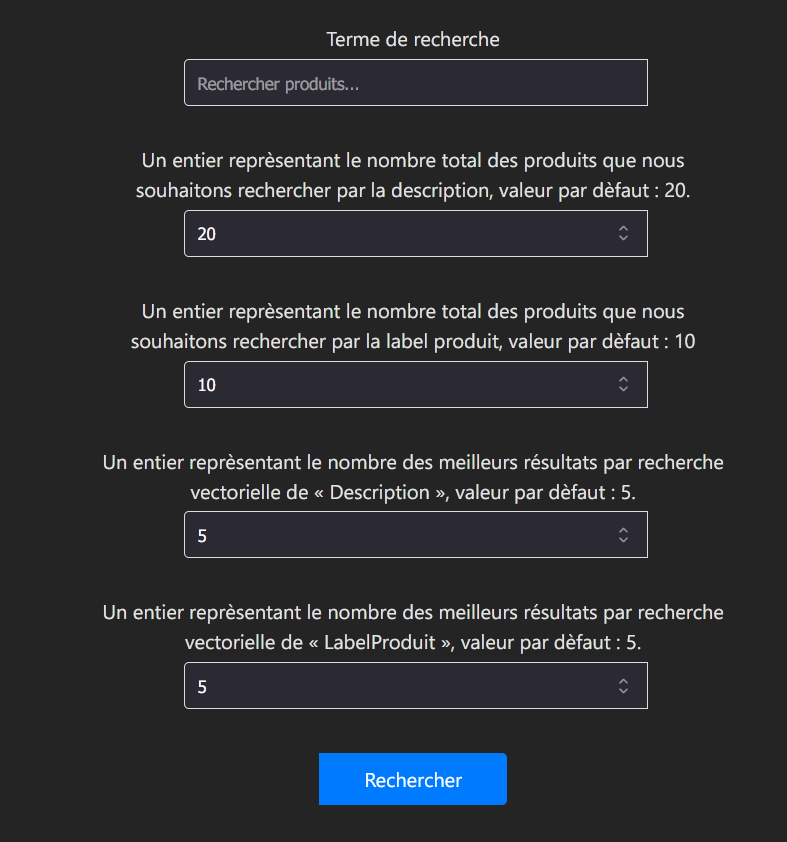
\includegraphics[width=1\textwidth]{logos/knnsearchform.png}
    \caption{Interface de modification de paramétres de recherche pour l'admin}
    \label{fig:knnsearchform}
\end{figure}

\newpage
\noindent
La figure ~\ref{fig:signin} illustre le formulaire d'authentification pour l'administrateur.

\begin{figure}[H]
    \centering
    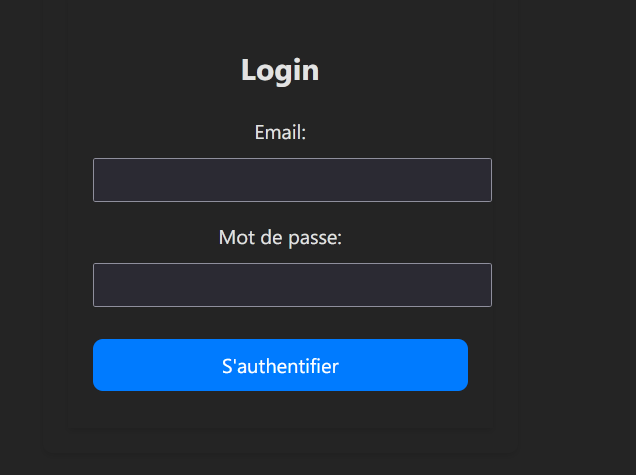
\includegraphics[width=1\textwidth]{logos/login.png}
    \caption{Interface de pour l'authentification de l'admin}
    \label{fig:signin}
\end{figure}

\section{Conclusion}
\noindent
Au terme du troisième sprint, nous avons réussi à intégrer un tableau de bord pour
l'administrateur dans notre application web. Cela permet à l'administrateur de mesurer et voir quelles termes de recherche donne les meilleurs résultats, ainsi que les termes de recherche les plus recherché sur notre site. Ainsi que modifier les paramétres de recherche des produits pour potntiellement améliorer la précision des résultats de recherche. Notre application est maintenant enrichi des fonctionnalités Business Intelligence.

